\subsection{Modell der Seite}
    % TODO: UML Diagramm der Seite, dann ist es auch ein Modell
    Abbildung \ref{image:findingNewsModelOverview} zeigt einen
    Ausschnitt der zu klassifizierenden Seite,
    anhand dessen das Modelld er Seite erläutert wird.
    Eine schematische Darstellung ist außerdem in Abbildung
    \ref{image:findingNewsModelUml} zu sehen.
    Aufgrund der nachfolgend beschriebenen Überschneidungen zum
    ersten Fallbeispiel, verzichtet dieses auf die Wiederholung
    identischer Elemente.

    \begin{figure}[htb]
        \centering
        
\includegraphics[width=\textwidth]{../resources/findings/case-study-2/news-overview.png}
        \caption{Ausschnitt aus einer Seite: Lehrende und Betreuende}
        \label{image:findingNewsModelOverview}
    \end{figure}

    Es ist leicht zu erkennen, dass es auf dieser Seite einige Überschneidungen
    mit der des vorherigen Beispiels gibt.
    Das betrifft den Kopfbereich, den Namen des Portals,
    die seitlichen Navigationspunkte und die Überschrift der Seite.
    Im Vergleich zum ersten Beispiel gibt es hier nur wenige inhaltliche,
    keine konzeptionellen Unterschide.

    Diese werden erst im mittleren Bereich ersichtlich,
    wo die Auflistung der einzelnen Nachrichten erfolgt.
    Jede Nachricht besitzt ein Datum, eine Überschrift und beliebig viele Absätze,
    die Text, Links etc. enthalten.
    Die Überschrift ist gleichzeitig auch ein Link auf die Einzelseite der Meldung.
    Diese Seite enthält nicht alle Meldungen.
    Stattdessen werden sie auf mehrere Seiten verteilt.
    Zwei Links, die in Abbildung \ref{image:findingNewsModelOverview} nicht zu sehen ist,
    führen einen Besucher der Webseite zur nächsten bzw. vorherigen Übersichtsseite.
    Dabei handelt es sich um eigenständige Seiten mit individuellen \glspl{url},
    die aber alle dem beschriebenen Modell folgen.

    \begin{figure}[htb]
        \centering
        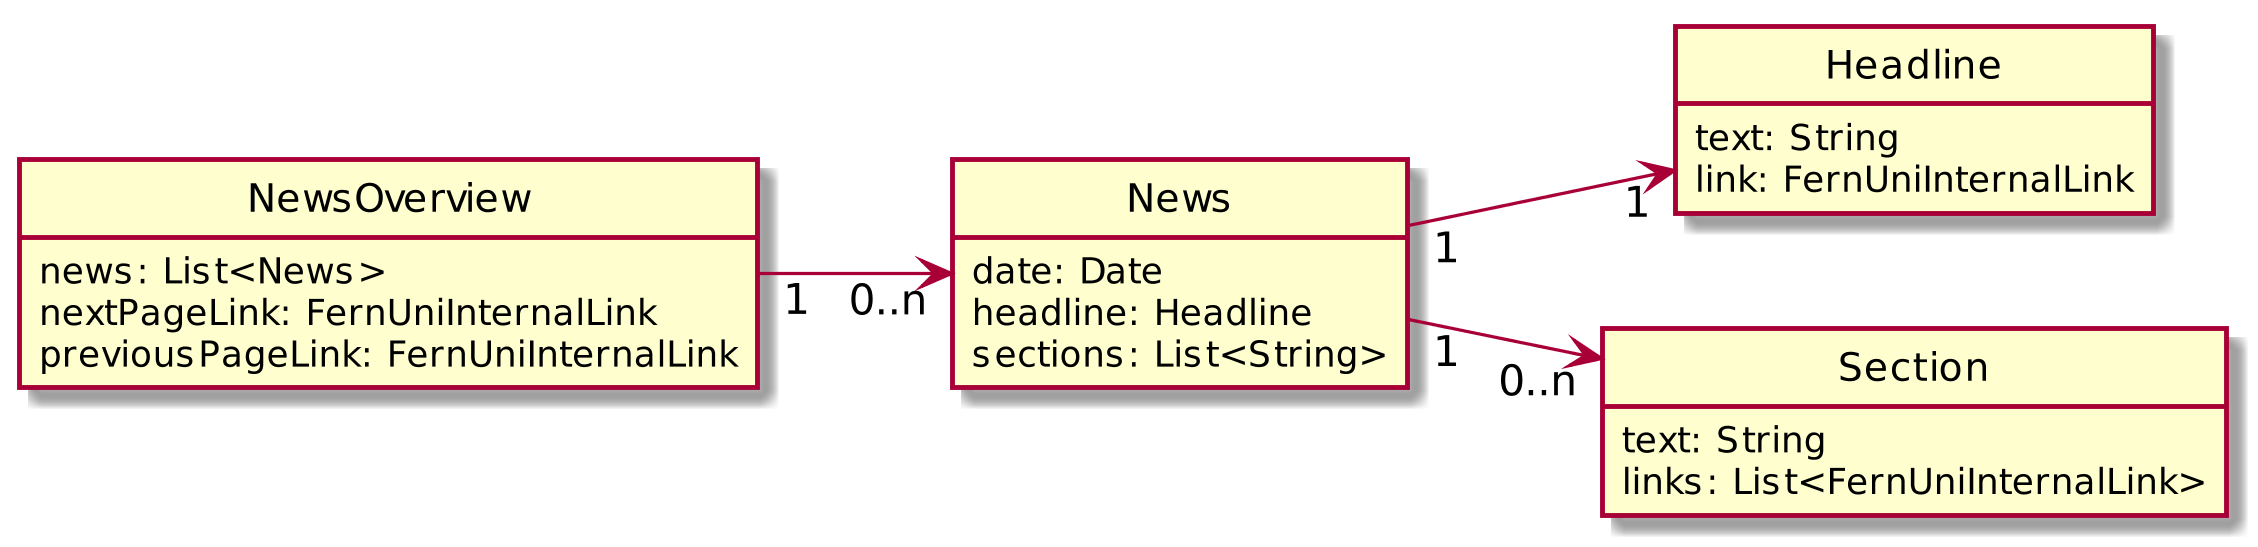
\includegraphics[width=\textwidth]{../resources/findings/case-study-2/model.png}
        \caption{Schematische Darstellung einer Nachrichtenübersichtsseite}
        \label{image:findingNewsModelUml}
    \end{figure}